\begin{appendices}
\addtocounter{chapter}{1}
\fancypagestyle{plain}{%
  \fancyhead[LO, RE]{\nouppercase{\rightmark}}
}
\renewcommand{\sectionmark}[1]{%
\markboth{\textbf{#1}}{}}

\section{Order Picking Process}
\vspace*{-2cm}
\begin{figure}[H]
	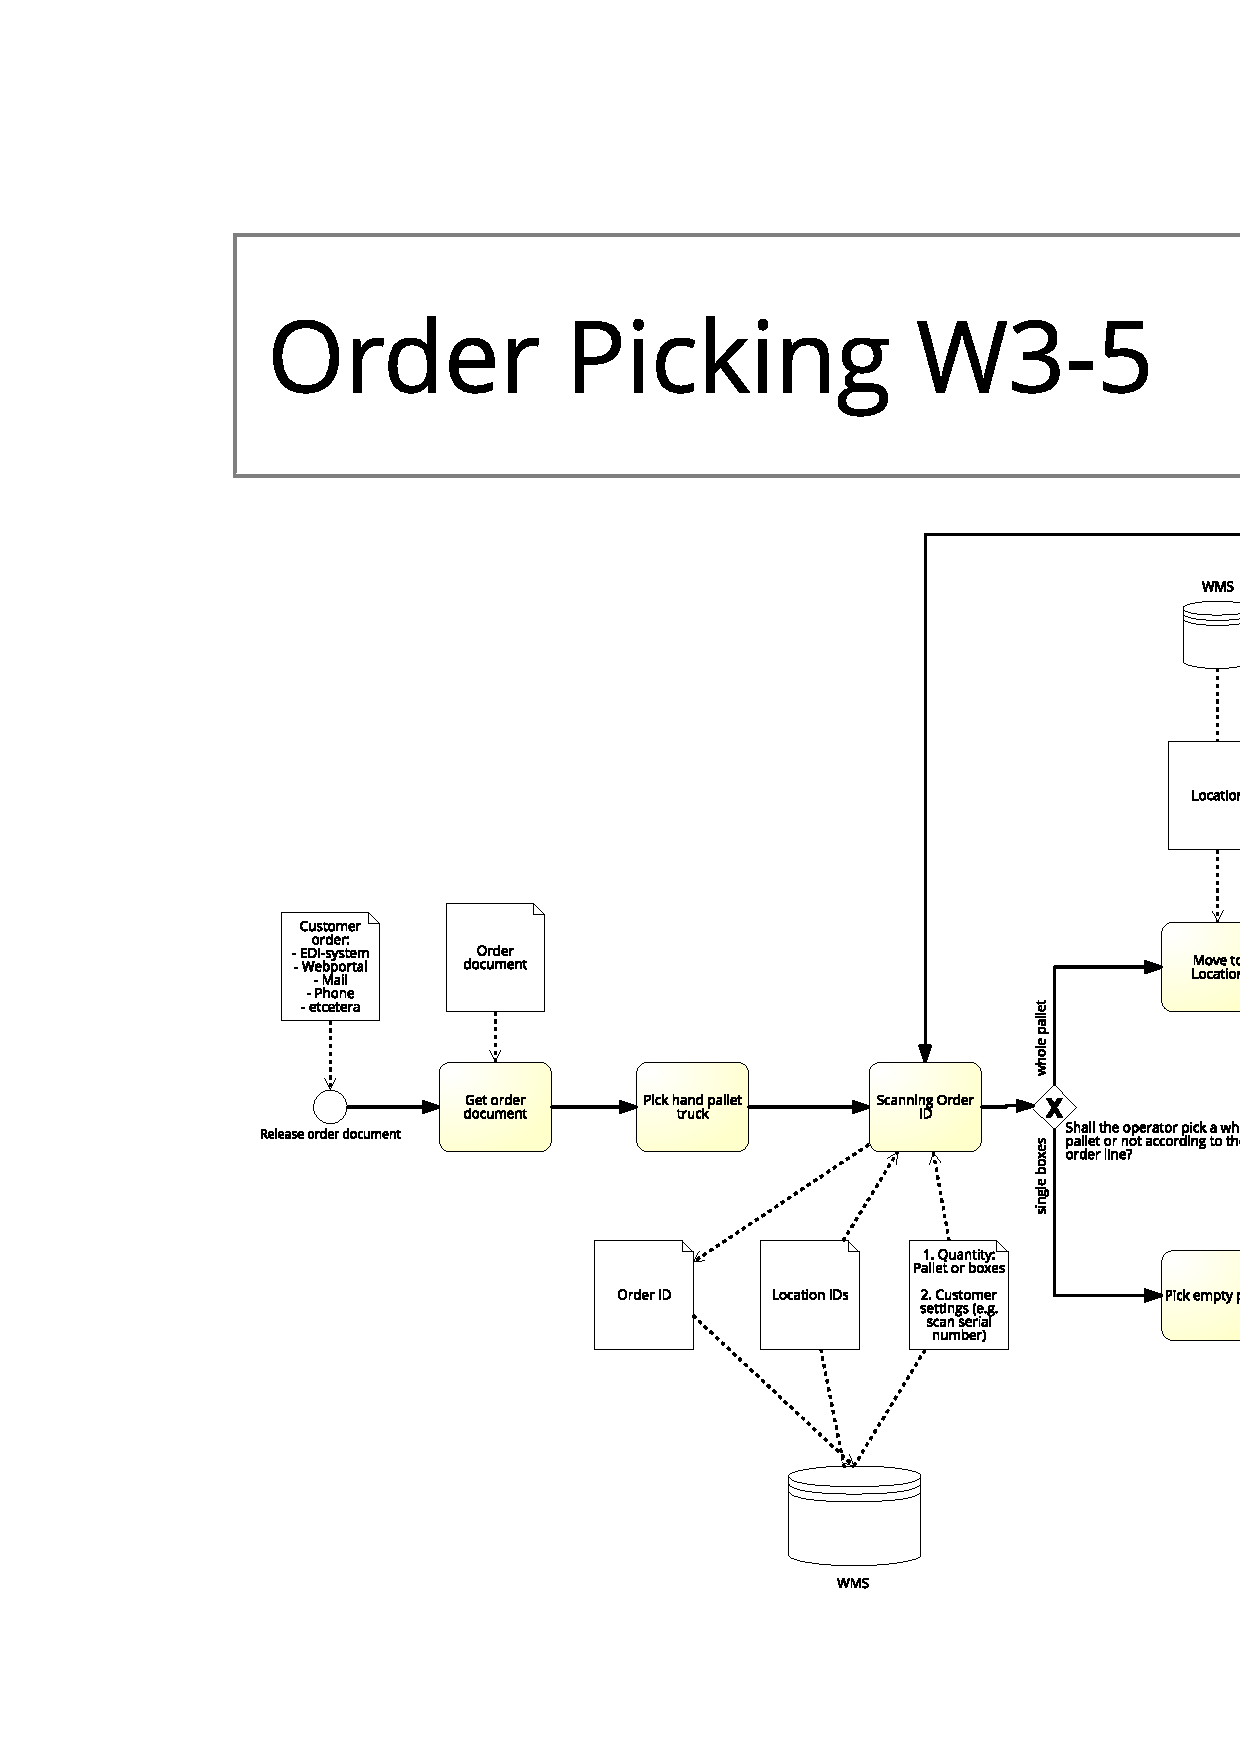
\includegraphics[width=\textwidth, page=1]{images/OrderPickingW3-5}
	\caption{Order Picking Process Diagram \citep{image:logwearOrderPicking}}
	\label{fig:orderPickingProcessDiagram}
\end{figure}
\begin{figure}\ContinuedFloat
	\includegraphics[width=\textwidth, page=2]{images/OrderPickingW3-5}
	\caption*{Figure \ref{fig:orderPickingProcessDiagram}: Order Picking Process Diagram \citep{image:logwearOrderPicking}}
\end{figure}
\begin{figure}\ContinuedFloat
	\includegraphics[width=\textwidth, page=3]{images/OrderPickingW3-5}
	\caption*{Figure \ref{fig:orderPickingProcessDiagram}: Order Picking Process Diagram \citep{image:logwearOrderPicking}}
\end{figure}
\begin{figure}\ContinuedFloat
	\includegraphics[width=\textwidth, page=4]{images/OrderPickingW3-5}
	\caption*{Figure \ref{fig:orderPickingProcessDiagram}: Order Picking Process Diagram \citep{image:logwearOrderPicking}}
\end{figure}

\clearpage

\section{Use Cases Reference Model} \label{sec:useCasesReferenceModel}

\begin{figure}[htbp]
	\begin{UseCase}{UC-W1}{Get Order (Voice)}{Wearable}{1.0}{LUR}
		\Actors{Picking Worker}
		\Description{A picking worker equipped with a wearable is using a voice command to get the next order displayed.}
		\Preconditions{The wearable has to be equipped with an Input Interface accepting voice and and an Output Interface that is able to return information to the user.}
		\Scenario{
			\vspace{0.1\baselineskip}
 		   \begin{enumerate*}
    			\item The Picking worker gives the voice command "Next Order".
    			\item The Wearable asks the WMS for the next order for the specific worker.
    			\item The WMS sends the Data to the Wearable
    			\item The Wearable displays the Data to the order picker.
			\end{enumerate*}
		}
		\Extensions{
			\vspace{0.1\baselineskip}
			\begin{enumerate*}
				\item[-]
			\end{enumerate*}
		}
		\Exceptions{
			\vspace{0.1\baselineskip}
			\begin{enumerate*}
				\item[1.1] The Voice command could not be properly understood. The Wearable does nothing.
				\item[1.2] The Order Picker is already on an Order and that one is unfinished, the command is ignored.
				\item[1.3] Another Voice command is understood, that one is executed.
				\item[3.1] The WMS did not find a next order. The order picker is informed about that.
				\item[4.1] There is an error in the format that was received. The data that could be understood is still displayed and the order picker is informed, that there might be an error with the order.
			\end{enumerate*}
		}
		\Result{The Order Picker has received the next order.}
	\end{UseCase}
	\caption{Use Case: Get Order(Voice)}
\end{figure}

\begin{figure}
	\begin{UseCase}{UC-W2}{Order Confirmation}{Wearable}{1.1}{LUR}
		\Actors{Picking Worker}
		\Description{A picking worker equipped with a wearable is using an input interface to confirm an order.}
		\Preconditions{The order picker has finished picking the order and wants to confirm that everything is correct.}
		\Scenario{
			\vspace{0.1\baselineskip}
		    \begin{enumerate*}
		    	\item The order picker uses an input interface on the Wearable to confirm the Order.
 		   	\item The wearable is processing the request.
 		   	\item The wearable is sending the Confirmation to the WMS.
 		   	\item The WMS sends, that the confirmation was successfully received.
		    	\item The wearable displays the user, that the confirmation was received by the WMS.
		    \end{enumerate*}
		}
		\Extensions{
			\vspace{0.1\baselineskip}
			\begin{enumerate*}
				\item[1.1] The Wearable is able to check if the confirmation is allowed to be send. See UC-W3.
			\end{enumerate*}
		}
		\Exceptions{
			\vspace{0.1\baselineskip}
			\begin{enumerate*}
				\item[3.1] The Wearable got an error when processing the request. The order picker is informed about the cause of the error and can try to fix it.
				\item[4.1] The WMS does not answer. The order picker is informed about that and can try contacting the IT.
			\end{enumerate*}
		}
		\Result{The Order Picker has confirmed his order.}
	\end{UseCase}
	\caption{Use Case: Order Confirmation}
\end{figure}


\begin{figure}
	\begin{UseCase}{UC-W3}{Order Control}{Wearable}{1.1}{LUR}
		\Actors{Picking Worker}
		\Description{A picking worker is in the process of picking his order.}
		\Preconditions{The wearable has a vision interface or is in another way able to control what the order picker is doing. Furthermore the order picker is currently in the process of picking an order and is picking a specific item of that order.}
		\Scenario{
			\vspace{0.1\baselineskip}
    		\begin{enumerate*}
    			\item The order picker scans an item.
		    	\item The wearable checks what is being packed.
		    	\item The order picker is putting the item on his hand pallet truck.
		    	\item The wearable is counting the amount of items put onto the hand pallet truck.
		    	\item The order picker scans a new item.
	 		   	\item The wearable detects a new item and ends the counting process for the last item.
	 		   	\item The wearable informs the order picker that everything went correctly with the last item.
    		\end{enumerate*}
		}
		\Extensions{
			\vspace{0.1\baselineskip}
			\begin{enumerate*}
				\item[6.1] When the order has no next item, the worker tries to confirm the order and the wearable can then proceed to check if the amount of picked parcels was correct.
			\end{enumerate*}
		}
		\Exceptions{
			\vspace{0.1\baselineskip}
			\begin{enumerate*}
				\item[7.1] The order picker could have counted wrongly and the wearable is informing him about it. After the order picker has checked the quantity on the Truck, go back to 1. with the item started with.
				\item[7.2] The wearable could have counted wrongly and the wearable is informing the order picker as if he counted wrong. The order picker can check the hand pallet truck for the item and confirm the right quantity.
				\item[7.3] The order picker could have picked the wrong quantity and the wearable could have counted wrong, resulting in the wearable saying the order picker has picked the right amount. An error is made.
			\end{enumerate*}
		}
		\Result{The Order Picker completed a part of the order and the wearable confirmed the quantity of that part.}
	\end{UseCase}
	\caption{Use Case: Order Control}
\end{figure}

\section{Web Application Mockups}\label{sec:webappmockups}
\begin{figure}[htbp]
	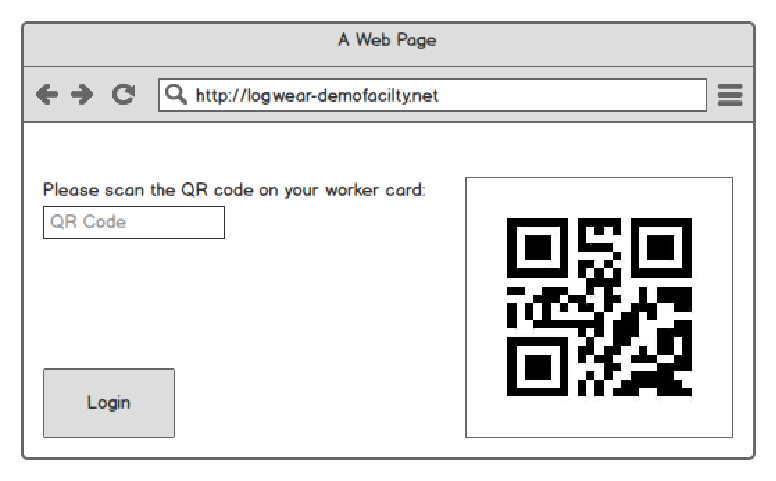
\includegraphics[width=\textwidth, page=1]{images/WebAppMockups}
	\caption{Mockup Worker Login}
\end{figure}
\begin{figure}
	\includegraphics[width=\textwidth, page=2]{images/WebAppMockups}
	\caption{Mockup No Order Started}
\end{figure}
\begin{figure}
	\includegraphics[width=\textwidth, page=3]{images/WebAppMockups}
	\caption{Mockup Start Order}
\end{figure}
\begin{figure}
	\includegraphics[width=\textwidth, page=4]{images/WebAppMockups}
	\caption{Mockup Confirm Order Line}
\end{figure}
\begin{figure}
	\includegraphics[width=\textwidth, page=5]{images/WebAppMockups}
	\caption{Mockup Confirm Order}
\end{figure}
\end{appendices}
